\documentclass[letterpaper,10pt]{article}

\usepackage{enumitem}
\usepackage{titling}
\usepackage{listings,listings-rust}
\usepackage{url}
\usepackage{soul}
\usepackage{hyperref}
\usepackage{setspace}
\usepackage{subfig}
\usepackage{sectsty}
\usepackage{pdfpages}
\usepackage{colortbl}
\usepackage{multirow}
\usepackage{multicol}
\usepackage{relsize}
\usepackage{amsmath}
\usepackage{wasysym}
\usepackage{fancyvrb}
\usepackage[yyyymmdd]{datetime}
\usepackage{amsmath,amssymb,amsthm,graphicx,xspace}
\usepackage[titlenotnumbered,noend,noline]{algorithm2e}
\usepackage[compact]{titlesec}
\usepackage{XCharter}
\usepackage[T1]{fontenc}
\usepackage[scaled]{beramono}
\usepackage[normalem]{ulem}
\usepackage{booktabs}
\usepackage{tikz}
\usetikzlibrary{arrows.meta,automata,shapes,trees,matrix,chains,scopes,positioning,calc,decorations.pathreplacing}
\tikzstyle{block} = [rectangle, draw, fill=blue!20, 
    text width=2.5em, text centered, rounded corners, minimum height=2em]
\tikzstyle{bw} = [rectangle, draw, fill=blue!20, 
    text width=4em, text centered, rounded corners, minimum height=2em]

\definecolor{namerow}{cmyk}{.40,.40,.40,.40}
\definecolor{namecol}{cmyk}{.40,.40,.40,.40}
\renewcommand{\dateseparator}{-}

\let\LaTeXtitle\title
\renewcommand{\title}[1]{\LaTeXtitle{\textsf{#1}}}

\lstset{basicstyle=\footnotesize\ttfamily,breaklines=true}

\newcommand{\CPP}{C\nolinebreak\hspace{-.05em}\raisebox{.4ex}{\tiny\bf +}\nolinebreak\hspace{-.10em}\raisebox{.4ex}{\tiny\bf +}}
\def\CPP{{C\nolinebreak[4]\hspace{-.05em}\raisebox{.4ex}{\tiny\bf ++}}}

\newcommand{\handout}[5]{
  \noindent
  \begin{center}
  \framebox{
    \vbox{
      \hbox to 5.78in { {\bf ECE459: Programming for Performance } \hfill #2 }
      \vspace{4mm}
      \hbox to 5.78in { {\Large \hfill #4  \hfill} }
      \vspace{2mm}
      \hbox to 5.78in { {\em #3 \hfill \today} }
    }
  }
  \end{center}
  \vspace*{4mm}
}

\newcommand{\lecture}[3]{\handout{#1}{#2}{#3}{Lecture #1}}
\newcommand{\tuple}[1]{\ensuremath{\left\langle #1 \right\rangle}\xspace}

\addtolength{\oddsidemargin}{-1.000in}
\addtolength{\evensidemargin}{-0.500in}
\addtolength{\textwidth}{2.0in}
\addtolength{\topmargin}{-1.000in}
\addtolength{\textheight}{1.75in}
\addtolength{\parskip}{\baselineskip}
\setlength{\parindent}{0in}
\renewcommand{\baselinestretch}{1.5}
\newcommand{\term}{Winter 2023}

\singlespace


\begin{document}

\lecture{28 --- Causal and Simulation Profiling}{\term}{Jeff Zarnett}

\section*{Causal Profiling}
At this point we've got some experience in identifying areas of the program that we think are slow or are limiting the maximum performance of our program. If we are presented with more than one thing, how do we know which of those would yield the most benefit? Is it possible that optimizing something would actually have no effect or even a negative effect? The scientific approach would be to do an experiment and find out. That is, change the code, see the impact, re-evaluate. What causal profiling offers us is a way to run those experiments without changing any code. That could be a significant savings of time and effort. 

One such causal profiler is called Coz (pronounced like ``cause'')~\cite{coz}. It does a what-if analysis that says: what would be the impact of speeding up this particular part of the code? 

A very simple approach would just look at the time of the program and just calculate what happens if the runtime of function \texttt{work()} is reduced by, say, 10\%. But that isn't a realistic approach, because speeding up that function might have no overall impact or change the execution time by increasing lock contention or some other mechanism. No, we actually need a simulation. 

The key observation of the Coz profiler authors is the idea that speeding up some area of code is fundamentally the same as slowing down every other part of the code. It's all relative! This is what we would call a virtual speedup. How is the other code slowed down? Adding some pauses to (stopping the execution of) the other threads. That certainly makes them run slower. Maybe you're not convinced that slowing down everything else is equivalent?


Shown below is the argument from~\cite{coz} in visual form. The original runtime is shown as (a). Hypothetically, say we make function \texttt{f} faster by some factor $d = 40\%$ that gives us (b). But, if instead of actually making function \texttt{f} faster, let's pause other threads for $0.4 \times t(f)$ where $t(f)$ is the original execution time of \texttt{f}. Then we get an equivalent effect to that of optimizing \texttt{f} by $d$.
\begin{center}
	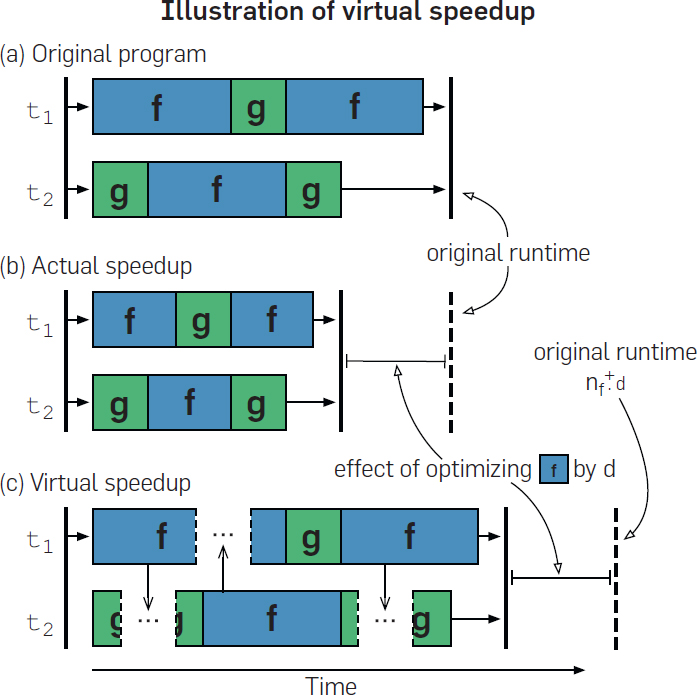
\includegraphics[width=0.4\textwidth]{images/virtual-speedup.jpg}
\end{center}

The tool provides some graphs of potential program speedup. From the recorded presentation, it might look something like the diagram below, where the boxes on the right correspond to different theoretical actions in the application being examined:

\begin{center}
	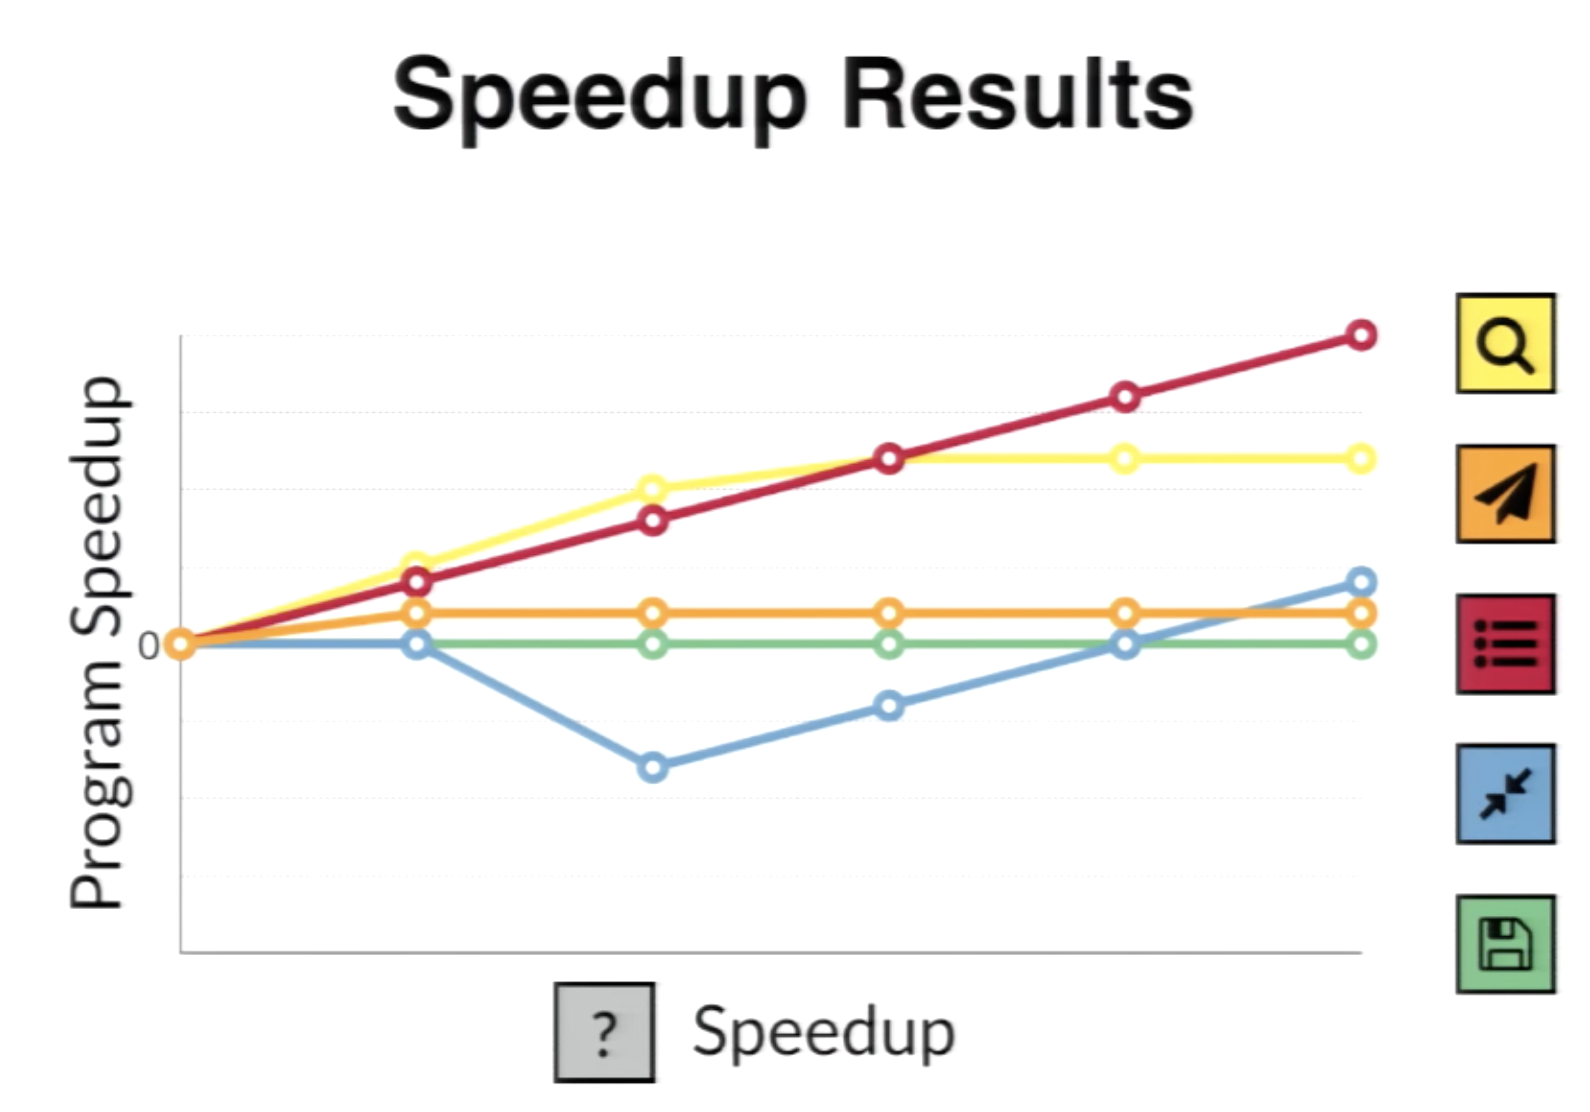
\includegraphics[width=0.4\textwidth]{images/coz-speedup-graph.png}
\end{center}

This pretend application shows all the possible outcomes, from continuous linear speedup, to speedup capped at some point, to no effect, and finally to where optimizing something makes the overall program runtime worse. 

It's easy to imagine scenarios corresponding to each of those. If we're computing the n-body problem, anything that improves the calculation of forces will certainly make things better. And it's easy to imagine that sometimes optimizing a part of the program does not improve anything because that code is not on the critical path. We can also easily imagine that improving something works up to a point where it ceases to be the limiting factor. But making things worse? We already covered that idea: speeding up a thread may increase lock contention or add something to the critical path. At some point, things may recover and be a net benefit.

It is important to remember that just because hypothetically speeding up a particular part of the program would be beneficial, doesn't mean that it's possible to speed up that part. And almost certainly not possible to do so to an arbitrary degree. We still have to make an assessment of what optimizations we can make and how difficult it would be to actually realize those improvements.

Once we've made a change to the program, then it's time to run an experiment again with the new baseline to see what else we can do.

The paper has a table summarizing the optimizations they applied to a few different programs, which seems to support the idea that the tool can be used effectively to get a meaningful speedup with relatively few lines of code~\cite{coz}:
\begin{center}
	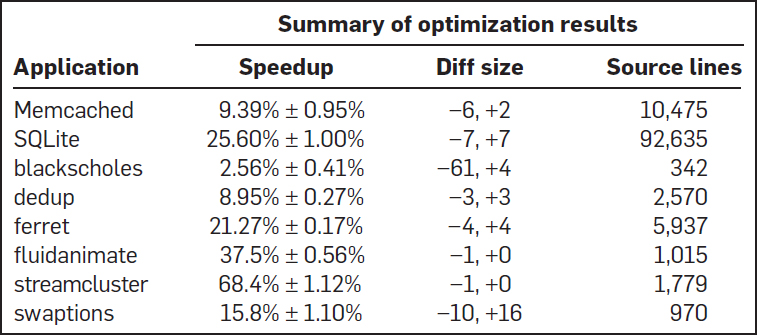
\includegraphics[width=0.6\textwidth]{images/coz-speedup.jpg}
\end{center}

There are potentially some limitations to this, of course. Putting pauses in the execution of the code can work when the execution of the program is all on the same machine and we have control over all the threads; it would need some meaningful extension to work for a distributed system where coordinating things across many servers would be needed.

Using some benchmarking workload, the authors estimate a 17.6\% overhead for this tool, which is broken down into 2.6\% for startup debug information collection, sampling at 4.8\%, and 10.2\% is the delay that's caused by slowing down other threads to create a virtual speedup~\cite{coz}.

If you'd like to see some more details of the tool, you can see the author presentation at the ACM symposium here: \url{https://www.youtube.com/watch?v=jE0V-p1odPg}

\subsection*{The Next Generation: SCOZ}
A few years later, another group of researchers worked to extend the Coz profiler to account for some limitations: inability to look at multi-process applications (which we just talked about), but also cases where the OS itself becomes a bottleneck~\cite{scoz}. You may recall that looking into the kernel is not always permitted for a given profiling tool -- depending on permissions.  It is therefore obvious to imagine that if one cannot look, then one cannot touch. 

If, indeed, the kernel is a bottleneck, it may or may not be possible to do very much about it. Avoiding system calls is one of the ``do less work'' strategies that you have likely already considered; oftentimes doing the system call is because we must. In an open-source OS or a kernel module we control, then we would have the ability to do something about it, if coz could give some recommendations.

The approach of~\cite{scoz} is to move from a thread-based system to a core-based one. So where, previously, to simulate speedup of a particular section of code the tool would pause all other threads, now it pauses execution on all other cores. There are some details to consider about what to do when there are idle cores to make sure that the delay is charged to the ``right'' core when one is woken up by another. The diagram the authors provides helps to explain it well:

\begin{center}
	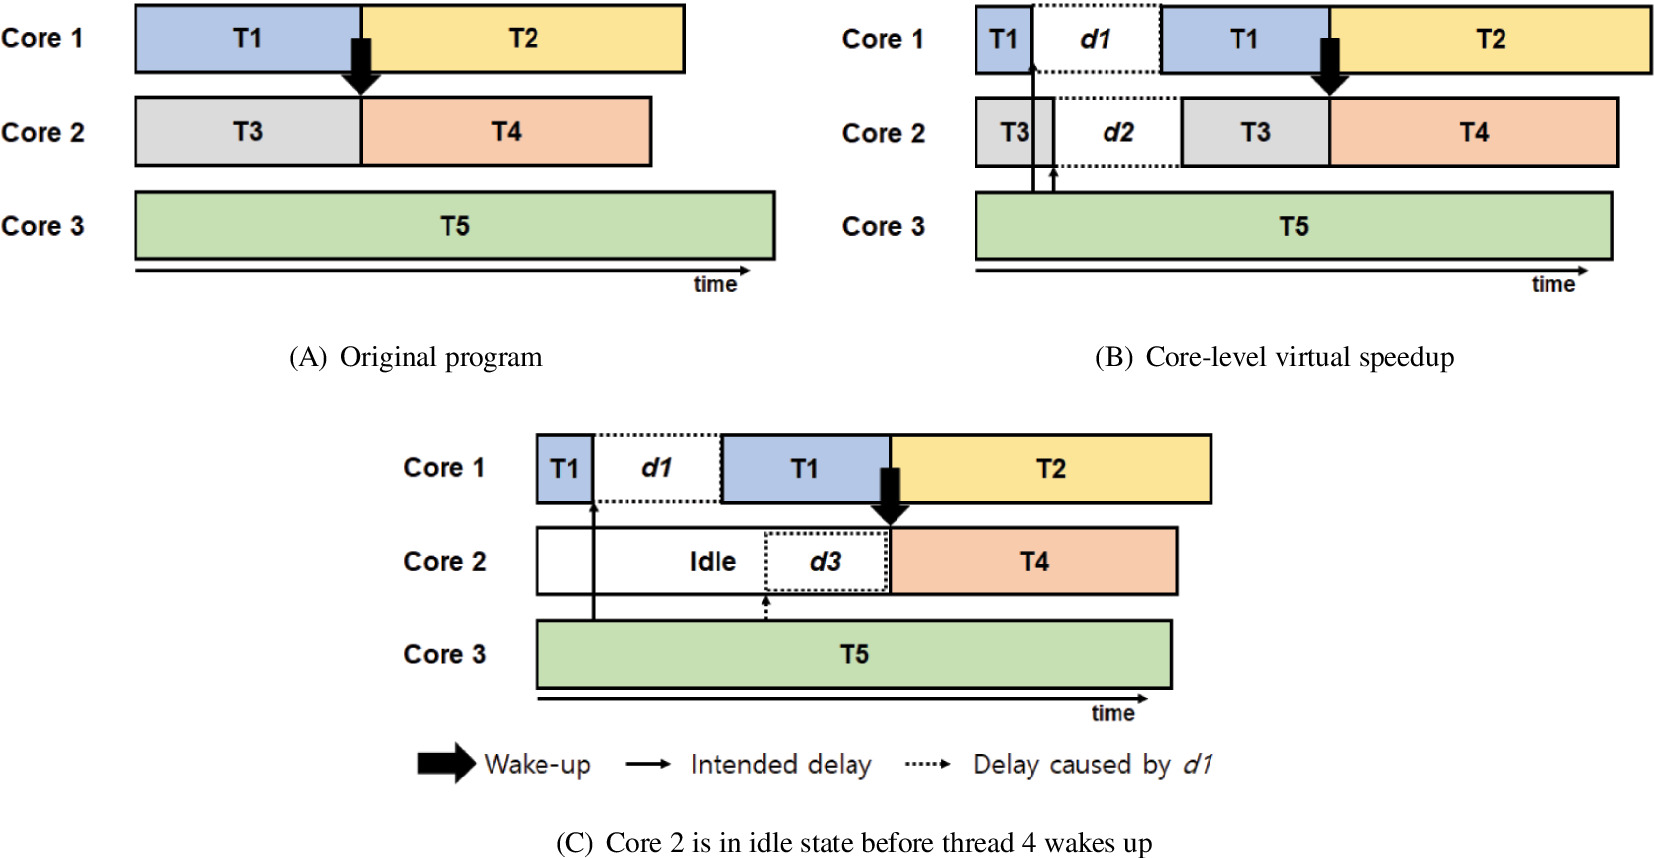
\includegraphics[width=0.8\textwidth]{images/scoz-delay.jpg}
\end{center}

The implementation involves one profiler thread for each core to manage its behaviour. The thread is pinned to the core, and its purpose is primarily to call the \texttt{ndelay} interface (with preemption temporarily disabled) to stop execution of code on that specific core~\cite{scoz}. 

This extension does allow \texttt{scoz} to do more than coz, but it does require running within the kernel, which imposes certain limitations to where and how it can be applied. That's an interesting tradeoff!

\section*{Simulations}
Causal profiling is a really neat idea in terms of using a simulation to make decisions. Other ways of using simulation for performance analysis exist! Let's talk about a couple examples.

\subsection*{Cachegrind}

Cachegrind is another tool in the Valgrind package and this one is much more performance oriented than the other two tools. Yes, memcheck and Helgrind look for errors in your program that are likely to lead to slowdowns (memory leaks) or make it easier to parallelize (spawn threads) without introducing errors. Cachegrind, however, does a simulation of how your program interacts with cache and evaluates how your program does on branch prediction. As we discussed earlier, cache misses and branch mispredicts have a huge impact on performance.

Recall that a miss from the fastest cache results in a small penalty (perhaps, 10 cycles); a miss that requires going to memory requires about 200 cycles. A mispredicted branch costs somewhere between 10-30 cycles. All figures \& estimates from the cachegrind manual~\cite{cachegrind}.

Cachegrind reports data about the First Level Instruction Cache (I1) [L1 Instruction Cache], the First Level Data Cache (D1) [L1 Data Cache], and the Last Level Cache (LL) [L3 Cache].

Unlike the normal Valgrind operation, you probably want to turn optimizations on (compile the release version). You still want debugging symbols, of course, but enabling optimizations will tell you more about what is going to happen in the released version of your program.

If I instruct cachegrind to run on a simple ECE 252-type example using the \texttt{--branch-sim=yes} option (because by default it won't show it):

\begin{lstlisting}
jz@Loki:~/ece254$ valgrind --tool=cachegrind --branch-sim=yes ./search
==16559== Cachegrind, a cache and branch-prediction profiler
==16559== Copyright (C) 2002-2013, and GNU GPL'd, by Nicholas Nethercote et al.
==16559== Using Valgrind-3.10.0.SVN and LibVEX; rerun with -h for copyright info
==16559== Command: ./search
==16559== 
--16559-- warning: L3 cache found, using its data for the LL simulation.
Found at 11 by thread 1 
Found at 22 by thread 3 
==16559== 
==16559== I   refs:      310,670
==16559== I1  misses:      1,700
==16559== LLi misses:      1,292
==16559== I1  miss rate:    0.54%
==16559== LLi miss rate:    0.41%
==16559== 
==16559== D   refs:      114,078  (77,789 rd   + 36,289 wr)
==16559== D1  misses:      4,398  ( 3,360 rd   +  1,038 wr)
==16559== LLd misses:      3,252  ( 2,337 rd   +    915 wr)
==16559== D1  miss rate:     3.8% (   4.3%     +    2.8%  )
==16559== LLd miss rate:     2.8% (   3.0%     +    2.5%  )
==16559== 
==16559== LL refs:         6,098  ( 5,060 rd   +  1,038 wr)
==16559== LL misses:       4,544  ( 3,629 rd   +    915 wr)
==16559== LL miss rate:      1.0% (   0.9%     +    2.5%  )
==16559== 
==16559== Branches:       66,622  (65,097 cond +  1,525 ind)
==16559== Mispredicts:     7,202  ( 6,699 cond +    503 ind)
==16559== Mispred rate:     10.8% (  10.2%     +   32.9%   )
\end{lstlisting}

So we see a breakdown of the instruction accesses, data accesses, and how well the last level of cache (L3 here) does.  Why did I say enable optimization? Well, here's the output of the search program if I compile with the \texttt{-O2} option. Yes, this was a C program, but the idea is the same.

\begin{lstlisting}
jz@Loki:~/ece254$ valgrind --tool=cachegrind --branch-sim=yes ./search
==16618== Cachegrind, a cache and branch-prediction profiler
==16618== Copyright (C) 2002-2013, and GNU GPL'd, by Nicholas Nethercote et al.
==16618== Using Valgrind-3.10.0.SVN and LibVEX; rerun with -h for copyright info
==16618== Command: ./search
==16618== 
--16618-- warning: L3 cache found, using its data for the LL simulation.
Found at 11 by thread 1 
Found at 22 by thread 3 
==16618== 
==16618== I   refs:      306,169
==16618== I1  misses:      1,652
==16618== LLi misses:      1,286
==16618== I1  miss rate:    0.53%
==16618== LLi miss rate:    0.42%
==16618== 
==16618== D   refs:      112,015  (76,522 rd   + 35,493 wr)
==16618== D1  misses:      4,328  ( 3,353 rd   +    975 wr)
==16618== LLd misses:      3,201  ( 2,337 rd   +    864 wr)
==16618== D1  miss rate:     3.8% (   4.3%     +    2.7%  )
==16618== LLd miss rate:     2.8% (   3.0%     +    2.4%  )
==16618== 
==16618== LL refs:         5,980  ( 5,005 rd   +    975 wr)
==16618== LL misses:       4,487  ( 3,623 rd   +    864 wr)
==16618== LL miss rate:      1.0% (   0.9%     +    2.4%  )
==16618== 
==16618== Branches:       65,827  (64,352 cond +  1,475 ind)
==16618== Mispredicts:     7,109  ( 6,596 cond +    513 ind)
==16618== Mispred rate:     10.7% (  10.2%     +   34.7%   )
\end{lstlisting}

Interesting results: our data and instruction miss rates went down marginally but the branch mispredict rates went up! Well sort of -- there were fewer branches and thus fewer we got wrong as well as fewer we got right. So the total cycles lost to mispredicts went down. Is this an overall win for the code? Yes. 

In some cases it's not so clear cut, and we could do a small calculation. If we just take a look at the LL misses (4~544 vs 4~487) and assume they take 200 cycles, and the branch miss penalty is 200 cycles, it went from 908~800 wasted cycles to 897~400; a decrease of 11~400 cycles. Repeat for each of the measures and sum them up to determine if things got better overall and by how much.

Cachegrind also produces a more detailed output file, titled \texttt{cachegrind.out.<pid>} (the PID in the example is 16618). This file is not especially human-readable, but we can ask the associated tool \texttt{cg\_annotate} to break it down for us, and if we have the source code available, so much the better, because it will give you line by line information. That's way too much to show even in the notes, so it's the sort of thing I can show in class (or you can create for yourself) but here's a small excerpt from the \texttt{search.c} example:



{\scriptsize
\begin{lstlisting}
--------------------------------------------------------------------------------
-- Auto-annotated source: /home/jz/ece254/search.c
--------------------------------------------------------------------------------
 Ir I1mr ILmr Dr D1mr DLmr Dw D1mw DLmw Bc Bcm Bi Bim 
127    1    1 96    3    0  4    0    0 23  11  0   0      for ( int i = arg->startIndex; i < arg->endIndex; ++i ) {
147    0    0 84    3    2  0    0    0 21   9  0   0          if ( array[i] == arg->searchValue ) {
  6    0    0  4    0    0  2    0    0  0   0  0   0              *result = i;
  2    0    0  0    0    0  0    0    0  0   0  0   0              break;
  .    .    .  .    .    .  .    .    .  .   .  .   .          }
  .    .    .  .    .    .  .    .    .  .   .  .   .      }
\end{lstlisting}
}

Cachegrind is very... verbose... and it can be very hard to come up with useful changes based on what you see... It may be better suited to something like quantifying whether a change has helped on some performance-critical code and why. The why (as in, mechanism) aspect is helpful in justifying to a manager or executive that the change you made actually solved the problem and the improved results are not just luck or measurement variance.

\subsection*{Simulation as Performance Debugging}
Simulation also allows for something that might be described as performance debugging. Executing in a simulation allows for more than just counting of the number of times that there is a cache miss or a pipeline stall -- you can see how we got there. That's helpful, even if it's not always actionable.

I got looking into some examples of this and came across some technical information for the TMS320C55x Digital Signal Processing platform by Texas Instruments.  I've never used it for anything and cannot honestly say anything about it. But the technical manual for its instruction set simulator\footnote{\url{https://www.ti.com/lit/ug/spru599d/spru599d.pdf}} has some interesting things to say about the value of simulation for profiling. Using a simulation approach, it's possible to get more exact values of how often something runs or count exactly how many cache misses, hits, and CPU stalls occur. Halting on an event trigger (e.g., pipeline stall) can give you lots of information about how to solve it without needing too much logging or tracing.

\subsection*{Interpreted Rust: Miri}
Despite sharing a name with an episode of the 1960s Star Trek where the \textit{Enterprise} comes across a planet that is an exact duplicate of earth, down to the continent layout and nobody seems to think that is an \textit{extremely big deal}, Miri is a profiling tool for Rust. It runs the Rust code in an interpreter which means it's slow, but helps in finding bugs. It shares a lot of similarities with Valgrind!

From reading its project description at \url{https://github.com/rust-lang/miri}, I think the real intended use of Miri is to detect issues in \texttt{unsafe} code. It is likely that in this course you've had only one situation where you really needed to use \texttt{unsafe} and that's launching a GPU computation, so its utility at first glance seems limited. But more complex programs in other scenarios may require more use of it. Miri seems to catch the sort of thing that we normally would find with Valgrind in other scenarios: array bounds violations, reading uninitialized memory, and memory leaks.

That's not all, though. Let's follow along an example of \cite{miri}, using Miri to generate some flamegraph-style results. To run, use the miri option and it will generate a \texttt{crox} directory with some file in it; process that file with the \texttt{crox} tool to generate a json file that can be read in chrome dev tools:

\begin{lstlisting}
MIRIFLAGS="-Zmiri-disable-isolation -Zmiri-measureme=crox" cargo +nightly miri run
\end{lstlisting}

Great! This produces a neat little flamegraph-style graph that shows what calls what and the time taken. If you prefer this to a flamegraph, that's perfectly fine. Both give you the same information in a similar way. The graphs are a bit much to show in the notes but screenshots in the slides help and we can do a live demo, too.

Much like Valgrind, it makes the program under observation run much, much slower. To make this work in a reasonable amount of time, I took the \texttt{producer-consumer-opt} code from earlier, but turned down the number of items per thread to 10 to try to not run out of patience before it produced the results. It gave some interesting graphs that you can poke around with. In the example run I have, you can see that for thread 1, initialization of the random number generator routine is quite slow and after that's happened, each subsequent use is quick. 


To be fair, the profiling-with-Miri article got a lot of comments that said things along the lines of ``maybe it's helping you to optimize the debug version, but most of the improvements will be done by compiling a release version''. That's acknowledged in the article with a callout that says that optimizing for Miri can have a negative impact on the actual performance, but at the very least Miri gives an idea of what it might make sense to change as part of the change-run-evaluate loop.

\input{bibliography.tex}

\end{document}
